\documentclass{article}
\usepackage{amsmath}
\usepackage{amssymb}
\usepackage{graphicx}
\usepackage{hyperref}
\usepackage[version=4]{mhchem}

\title{Problem 7}
\date{}

\begin{document}
\maketitle

\section*{Problem}
\(A B C D\) is a quadrilateral with \(A D / / B C\). Draw \(A G \perp A B\) to meet \(D C\) at \(F\) and the extension of \(B C\) at \(G\). Points \(E\) is the midpoint of sides \(B G\). Find the length \(A E\) if \(A D=\) 2.7, \(A F=4\), and \(A B=6\).\\
\centering
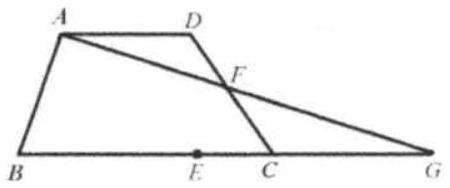
\includegraphics[width=\textwidth]{images/problem_image_1.jpg}

\section*{Solution}
5.\\
Draw \(A E\). Since \(A E\) is the median, by Theorem \(1.3, A E=B E=E G\).

Since \(A D / / B C, \angle D A F=\angle C G F\).\\
\centering
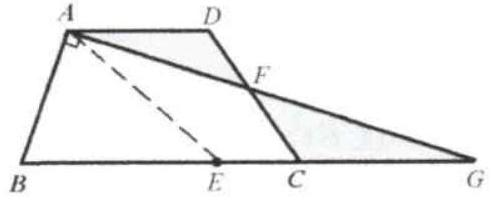
\includegraphics[width=\textwidth]{images/reasoning_image_1.jpg}\\
\(\angle D F A=\angle C F G\) (vertical angles).\\
\(\angle A D F=\angle G C F\).\\
Thus \(\triangle A D F \cong \triangle G C F . A F=F G=4\).\\
Triangle \(A B G\) is a \(6-8-10\) right triangle. \(B E=\frac{1}{2} B G=5\).\\
The answer is \(A E=B E=5\).

\end{document}
